\section{Risultati}\label{sec:risultati}

\subsection{Mean-field approximation}\label{subsec:res-mean-field-approximation}
    La mean-field approximation è un metodo per approssimare il comportamento 
    di un sistema complesso,semplificando le interazioni tra le entità coinvolte.
    Questo metodo è utile per studiare il comportamento del sistema in condizioni di equilibrio, ma non tiene conto
    dell'effetto delle fluttuazioni locali.
    Come possiamo vedere dalla figura ~\ref{fig:mf_critical_j}, il calcolo del campo medio approssima bene il valore
    critico di $J$, sia nel caso teorico che in quello pratico, confermando la validità teorica del metodo.

    \begin{figure}[h]
        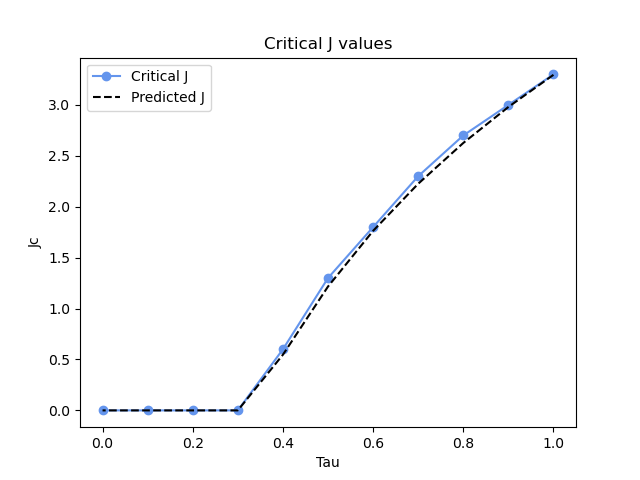
\includegraphics[width=\textwidth]{mf_critical_j}\caption{Mean-field approximation}
        \label{fig:mf_critical_j}
    \end{figure}

\subsection{Simple percolation}\label{subsec:res-simple-percolation}
    La simple percolation è un metodo per studiare la connettività di un sistema, considerando la probabilità di
    connessione tra i nodi.
    In questo caso, il modello SIR è stato approssimato con un modello di percolazione, in cui i nodi rappresentano le
    persone e i link rappresentano i contatti tra le persone.
    Questo metodo è utile per studiare la diffusione di una malattia in una rete, ma non tiene conto della percezione
    del rischio.
    Anche in questo caso, sia per la valutazione del valore critico di $J$ ottenuto dalla teoria che per quello
    ottenuto dalla pratica, il metodo si è dimostrato valido.
    In questa valutazione, abbiamo fatto varie simulazioni in base al numero di nodi e al valore di connettività $k$.
    I risultati mostrati in ~\ref{fig:prob_percolation} e ~\ref{fig:prob_percolation_2} mostrano i risultati ottenuti.

    \begin{figure}[h]
        \begin{minipage}{0.5\textwidth}
            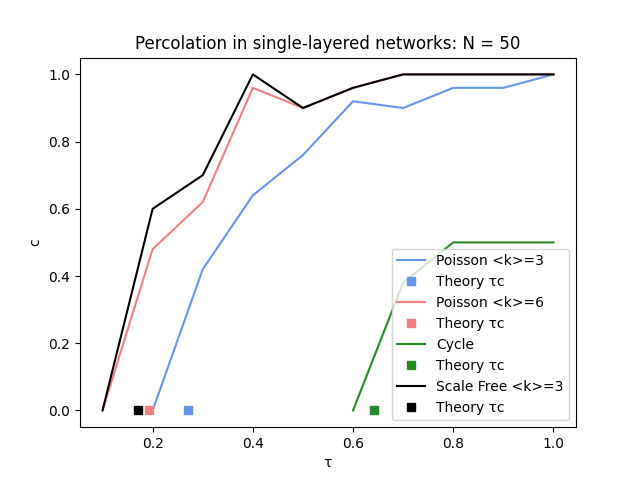
\includegraphics[width=\linewidth]{critical_t}\label{fig:prob_percolation}
        \end{minipage}
        \begin{minipage}{0.5\textwidth}
            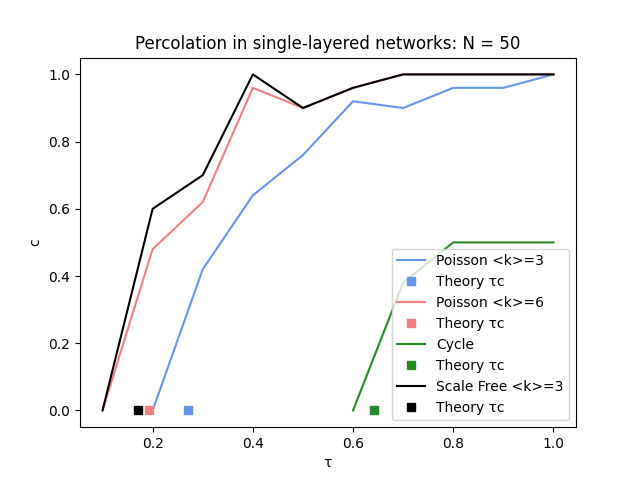
\includegraphics[width=\linewidth]{critical_t}\label{fig:prob_percolation_2}
        \end{minipage}
        \caption{Valutazione della probabilità di percolazione}
    \end{figure}

\subsection{Infezione con la percezione del rischio}\label{subsec:res-infezione-con-la-percezione-del-rischio}
    Il modello di infezione con la percezione del rischio tiene conto del fatto che le persone possono adottare misure
    precauzionali per proteggersi da una malattia.
    In questo caso, il modello SIR è stato esteso per includere la percezione del rischio, in modo che le persone possano
    adottare misure precauzionali in base alla loro percezione del rischio.
    Questo metodo è utile per studiare l'effetto della percezione del rischio sulla diffusione di una malattia, ma non
    tiene conto dell'effetto delle informazioni virtuali.

\subsection{Multiplex networks}\label{subsec:res-multiplex-networks}
    Le multiplex networks sono reti che consistono in più strati, o livelli, di connessioni tra i nodi.
    In questo caso, il modello SIR è stato esteso per includere una rete multiplex, in cui i nodi possono essere connessi
    in più strati di connessioni.
    Questo metodo è utile per studiare l'interazione tra la percezione del rischio e la diffusione di una malattia, ma
    richiede un'analisi più complessa per tener conto di tutti gli effetti.
    I risultati ottenuti dalla simulazione del modello multiplex sono mostrati in figura ~\ref{fig:diagram_phase}.
    Possiamo vedere come all'aumentare di $t$ e $q$ l'infezione si diffonde e non si è in grado di fermarla, infatti i
    valori di $Jc$ aumentano notevolmente.
    Nella visualizzazione del diagramma di fase, possiamo vedere come la diffusione mostri un andamento parabolico.

    \begin{figure}[h]
        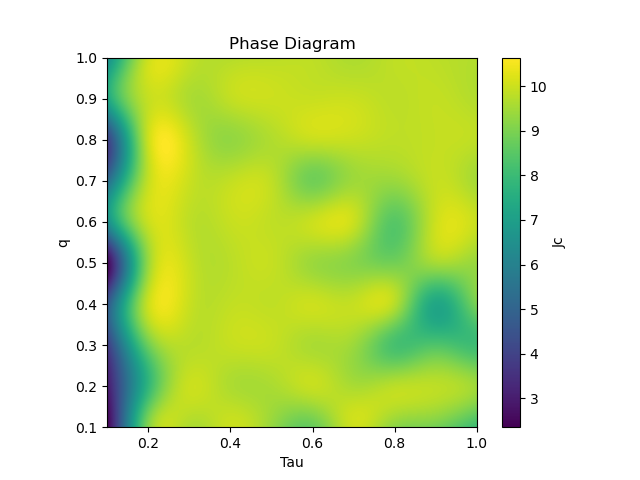
\includegraphics[width=\textwidth]{q_plot}\label{fig:diagram_phase}
        \caption{Diagramma di fase}
    \end{figure}
